\documentclass{Class}
\usepackage[utf8]{inputenc}
\usepackage{graphicx}
\usepackage{listings}
\usepackage{color}
\usepackage{float}
\usepackage{amsmath} 
\usepackage{hyperref}
% \usepackage{calrsfs}
\usepackage{mathrsfs}
\usepackage{aligned-overset}
\usepackage{amssymb}
\usepackage{mathtools}
\usepackage[mathscr]{euscript}
\usepackage{tikz}
\usepackage{bbm}
\usepackage[most]{tcolorbox}
\usepackage{booktabs}
\usepackage{amsthm}
\newcommand{\N}{\mathbb{N}}
\newcommand{\Q}{\mathbb{Q}}
\newcommand{\R}{\mathbb{R}}
\newcommand{\C}{\mathbb{C}}
\newcommand{\F}{\mathbb{F}}
\newcommand{\E}{\mathbb{E}}
\newcommand{\1}{\mathbbm{1}}
\newcommand{\X}{\mathsf{X}}
\newcommand{\Y}{\mathsf{Y}}
\newcommand{\B}{\mathcal{B}}
\newcommand{\lclass}{\mathcal{L}}
\newcommand{\Prob}{\mathbb{P}}
\newcommand{\deriv}{\mathrm{~d}}
\newcommand{\icomp}{\operatorname{i}}
\newcommand{\varx}{\varphi_\X}
\newcommand{\pfield}{(\Omega, \mathcal{F}, P)}
\newcommand \independent{\protect\mathpalette{\protect\independenT}{\perp}}
\def\independenT#1#2{\mathrel{\rlap{$#1#2$}\mkern2mu{#1#2}}}
\newtheorem{theorem}{Theorem}[subsection]
\newtheorem{definition}[theorem]{Definition} 
\newtheorem{lemma}[theorem]{Lemma} 
\newtheorem{corollary}[theorem]{Korollar} 
\newtheorem{remark}[theorem]{Bemærkning} 
\newtheorem{proposition}[theorem]{Sætning} 
\newtheorem{example}[theorem]{Eksempel}
\newtheorem{manualtheorem}{Theorem}
\newenvironment{theorem-manual}[1] 
  {\renewcommand\themanualtheorem{#1}\manualtheorem}
  {\endmanualtheorem}
  \newtheorem{manualprop}{Proposition}
  \newenvironment{prop-manual}[1] 
    {\renewcommand\themanualprop{#1}\manualprop}
    {\endmanualprop}

    \newlength{\leftstackrelawd}
    \newlength{\leftstackrelbwd}
    \def\leftstackrel#1#2{\settowidth{\leftstackrelawd}%
    {${{}^{#1}}$}\settowidth{\leftstackrelbwd}{$#2$}%
    \addtolength{\leftstackrelawd}{-\leftstackrelbwd}%
    \leavevmode\ifthenelse{\lengthtest{\leftstackrelawd>0pt}}%
    {\kern-.5\leftstackrelawd}{}\mathrel{\mathop{#2}\limits^{#1}}}
\usepackage{geometry}
    \geometry{
        a4paper,
        left=3.5cm,
        right=3.5cm   ,
    }
\definecolor{dkgreen}{rgb}{0,0.6,0}
\definecolor{gray}{rgb}{0.5,0.5,0.5}
\definecolor{mauve}{rgb}{0.58,0,0.82}
\newtcolorbox{theorem-box}{
    colback=gray!10, % Light grey background
    colframe=black,  % Black frame
    sharp corners,   % Square corners
    boxrule=0.8pt,   % Border thickness
    before skip=10pt, % Space before the box
    after skip=10pt,  % Space after the box
}

\newtheoremstyle{boxed}  % Define a new theorem style
  {10pt}   % Space above
  {10pt}   % Space below
  {}       % Body font
  {}       % Indent amount
  {\bfseries} % Theorem head font (bold)
  {.}      % Punctuation after theorem head
  { }      % Space after theorem head
  {\thmname{#1}~\thmnumber{#2}\textbf{\thmnote{ (#3)}}}  % Theorem head spec

\theoremstyle{boxed}
\lstset{frame=tb,
  language=Python,
  aboveskip=3mm,
  belowskip=3mm,
  showstringspaces=false,
  columns=flexible,
  basicstyle={\small\ttfamily},
  numbers=none,
  numberstyle=\tiny\color{gray},
  keywordstyle=\color{blue},
  commentstyle=\color{dkgreen},
  stringstyle=\color{mauve},
  breaklines=true,
  breakatwhitespace=true,
  tabsize=3
}
\renewcommand{\thesubsection}{\thesection.\arabic{subsection}}
\usetikzlibrary {shapes ,arrows , positioning }
\author{Markus Hohwü Larsen - 202205800}
\title{Assignment 1}
\begin{document}
\problem{1}
Consider i.i.d. real random variables $Y_1, Y_2, \ldots$ with common density $f$ given by

$$
f(y)= \begin{cases}\frac{1}{2} e^{-y}, & y \geq 0 \\ e^{2 y} & y<0\end{cases}
$$


Let $S_0=0$ and define $\left(S_n\right)_{n \geq 1}$ as

$$
S_n=Y_1+\cdots+Y_n, \quad \text { for } n \in \mathbb{N}
$$


Also define

$$
\mathcal{F}_n= \begin{cases}\{\emptyset, \Omega\} & \text { for } n=0 \\ \sigma\left(Y_1, \ldots, Y_n\right) & \text { for } n \in \mathbb{N}\end{cases}
$$
\begin{enumerate}
    \item For $n \in \mathbb{N}_0$ determine $\mathbb{E}\left[e^{\alpha S_{n+1}} \mid \mathcal{F}_n\right]$ for all $\alpha \in \mathbb{R}$.
    \item Determine $\mathbb{P}\left(S_n<0<S_{n+1} \mid \mathcal{F}_n\right)$ for $n \in \mathbb{N}$.
\end{enumerate}
\solution
\begin{enumerate}
    \item Let $n\in\N_0$, 
    $$\begin{aligned}
        \E[e^{\alpha S_{n+1}}|\mathcal{F}_n]&=\E[e^{\alpha(Y_1+\cdots + Y_n+Y_{n+1})}|\mathcal{F}_n]\\
        &=\E[e^{\alpha (Y_1+\cdots +Y_n)}e^{\alpha Y_{n+1}}|\mathcal{F}_n]\\
        &\leftstackrel{D.10(6)}{=} e^{\alpha (Y_1+\cdots +Y_n)}\E[e^{\alpha Y_{n+1}}|\mathcal{F}_n]\\
        &\leftstackrel{D.10(8)}{=}  e^{\alpha (Y_1+\cdots +Y_n)}\E[e^{\alpha Y_{n+1}}]\\
        &\leftstackrel{LOTUS}{=} e^{\alpha (Y_1+\cdots +Y_n)}\lim_{n\rightarrow \infty}\int_{-n}^{n}e^{\alpha y}f(y) \deriv y\\
        &= e^{\alpha (Y_1+\cdots +Y_n)}\left(\lim_{n\rightarrow \infty}\int_{-n}^{0}e^{\alpha y}e^{2y}\deriv y+\lim_{n\rightarrow \infty}\int_{0}^{n}e^{\alpha y}\frac{1}{2}e^{-y}\deriv y \right)\\
        &= e^{\alpha S_n}\left(\lim_{n\rightarrow \infty}\int_{-n}^{0}e^{\alpha y}e^{2y}\deriv y+\lim_{n\rightarrow \infty}\int_{0}^{n}e^{\alpha y}\frac{1}{2}e^{-y}\deriv y \right)\\
    \end{aligned}$$
    For $\lim_{n\rightarrow \infty}\int_{-n}^{0}e^{\alpha y}e^{2y}$ we have:
    $$\begin{aligned}
        \lim_{n\rightarrow n}\int_{-\infty}^{0}e^{\alpha y}e^{2y} &= \int_{-\infty}^{0}e^{(\alpha+2)y}\\
        &= \lim_{n\rightarrow \infty}\left[\frac{e^{(\alpha+2)y}}{\alpha+2}\right]^{0}_{-n}\\
        &= \begin{cases}
            \frac{1}{\alpha+2}, \; &\text{if }\alpha>-2\\
            \infty, \; &\text{otherwise}
        \end{cases}
    \end{aligned}$$
    For $\lim_{n\rightarrow \infty}\int_{0}^{n}e^{\alpha y}\frac{1}{2}e^{-y}\deriv y$ we have:
    $$
    \begin{aligned}
        \lim_{n\rightarrow \infty}\int_{0}^{n}e^{\alpha y}\frac{1}{2}e^{-y}\deriv y &= 2\int_{0}^{\infty}e^{(\alpha-1)y}\deriv y\\
        &=\frac{1}{2}\lim_{n\rightarrow \infty}\left[\frac{e^{(\alpha-1)}y}{\alpha-1}\right]_{0}^{n}\\
        &=\begin{cases}
            \frac{1}{2\alpha-2}, \; &\text{if }\alpha < 1\\
            \infty, \; &\text{otherwise}
        \end{cases}\\
    \end{aligned}
    $$
    Combining these we get:
    $$\mathbb{E}\left[e^{\alpha S_{n+1}} \mid \mathcal{F}_n\right] = \begin{cases}
        e^{\alpha S_n}\left(\frac{1}{\alpha+2}+\frac{1}{2\alpha-2}\right), &\text{if }-2<\alpha<1\\
        \infty, &\text{otherwise}
    \end{cases}$$
    \item Let $n\in\N$:
    $$
    \begin{aligned}
        \Prob(S_n<0<S_{n+1}|\mathcal{F}_n)\; &\leftstackrel{D.1(4)}{=}\E[\1_{\{S_n<0<S_{n+1}\}}|\mathcal{F}_n]\\
        &= \E[\1_{\{S_n<0\}}\1_{\{0<S_{n+1}\}}|\mathcal{F}_n]\\
        &= \E[\1_{\{S_n<0\}}\1_{\{-S_n<Y_{n+1}\}}|\mathcal{F}_n]\\
        &\leftstackrel{\independent}{=} \1_{\{S_n<0\}}\E[\1_{\{-S_n<Y_{n+1}\}}|\mathcal{F}_n]\\
        &\leftstackrel{D.7}{=} \1_{\{S_n<0\}}\E[\1_{\{-s<Y_{n+1}\}}|\mathcal{F}_n]\big{|}_{s=S_n}\\
        &=\1_{\{S_n<0\}}\lim_{n\rightarrow \infty}\int_{-s}^{n}\frac{1}{2}e^{-y}\deriv y\\
        &=\1_{\{S_n<0\}}\frac{e^s}{2}\\
        &=\begin{cases}
            \frac{e^{S_n}}{2}, &\text{if }S_n<0\\
            0, &\text{otherwise}
        \end{cases}
    \end{aligned}
    $$
\end{enumerate}



\problem{2}
Let the state space be $S=\mathbb{N}_0=\{0,1, \ldots\}$ and for $i \in S$ let $p_i \in[0,1]$. Consider the Markov chain with state space $S$ specified as follows: A particle which in state $i \in S$ moves to state $i+1$ in one step with probability $p_i$ and to state 0 with probability $1-p_i$
\begin{enumerate}
    \item Argue that the chain is irreducible if $p_i \in(0,1)$ for all $i \in S$. Also, indicate the transition diagram in this case.
    \item Determine $p_{02}^4$. For $n \in \mathbb{N}$ determine $\mathbb{P}_0\left(T_0 \geq n\right)$ and $\mathbb{P}_0\left(T_0=n\right)$.
    \item Show that state 0 is recurrent if and only if $\prod_{i=0}^{\infty} p_i=0$.
    \item Give a concrete example of probabilities $\left(p_i\right)_{i=0}^{\infty}$ such that $p_i \in(0,1)$ for all $i \in S$ and the chain is transient.
    \item Assume that $p_i \in(0,1)$ for all $i \in S$. Show that there exists a unique stationary distribution if and only if $\sum_{n=0}^{\infty}\left(p_0 p_1 \cdots p_n\right)<\infty$. Determine the stationary distribution when it exists.
\end{enumerate}
\solution
\begin{enumerate}
    \item To argue that the chain is irreducible, we need to argue that any state can be reached from any other state with positive probability.
    \\If $p_i\in(0,1)\forall i\in S$, we have probability $p_i>0$ for moving to state $i+1$ and probability $1-p_i>0$ for moving to state $0$.
    \\For states $i,j,$ we have that if $j>i,$ then to go from $i$ to $j$ we can move from $i$ to $i+1,i+2,\ldots, j$, with positive probability. If $j<i$ we can move to 0 from any state (with positive probability) and then move to state $1,2,\ldots, i$ with positive probability. As this covers all cases, the chain is irreducible. Here is a sketch for the transition digram:
    \begin{center}
        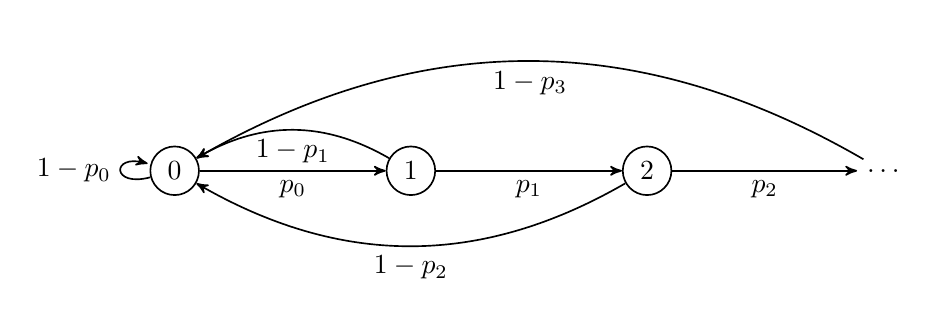
\begin{tikzpicture}[->, >=stealth', auto, semithick, node distance=3cm]
        \tikzstyle{every state}=[fill=white,draw=black,thick,text=black,scale=1]
        \node[circle, draw]    (A)                     {$0$};
        \node[circle, draw]    (B)[right of=A]   {$1$};
        \node[circle, draw]    (C)[right of=B]   {$2$};
        \node[]    (D)[right of=C]   {$\ldots$};
        \path
        (A) edge[loop left]			node{$1-p_0$}	(A)
            
        edge[below] node{$p_0$} (B)
        (B) edge[bend right,below]	node{$1-p_1$}	(A)
        
        edge[below]		node{$p_1$}	(C)
        (C) edge[bend left,below]	node{$1-p_2$}	(A)
        edge[below]		node{$p_2$}	(D)
        (D) edge[bend right, below]		node{$1-p_3$}	(A);
        \end{tikzpicture}
    \end{center}
    \item We want to determine to probability to go from state $0$ to state $2$ in exactly $4$ steps. There are only 2 combinations where this is possible as represented by the following paths:
    $$0\rightarrow 1\rightarrow  0 \rightarrow 1\rightarrow 2
    $$ with probability $p_0^2p_1(1-p_1)$, or
    $$0\rightarrow 0\rightarrow  0 \rightarrow 1\rightarrow 2$$
    with probability $(1-p_0)^2p_0p_1$, \\So we have that $$p_{02}^4=p_0^2p_1(1-p_1)+(1-p_0)^2p_0p_1$$
\\We now calculate $\Prob_0(T_0\geq n)$ and $\Prob_0(T_0=n)$. Let $n\in\N$. $T_0$ is the return time to state 0, meaning that if $T_0=n$ then we move to state 0 at time $n-1$ from a state $i$:
    \\For $\Prob_0(T_0\geq n)$, we want to calculate the probability of the first return time being at $n$ or later, if we start in state 0, i.e. not returning to 0 for the first $n-2$ steps and then no restrictions from time $n-1$ and onwards. Intuitively this is 
    $$\Prob_0(T_0\leq n)=\prod_{i=0}^{n-2}p_i$$
    For $\Prob_0(T_0= n)$ we want the probability of the first return time being exactly at time $n$. This is the same as not returning for the first $n-2$ steps and then exactly returning at the $n-1'th$ step
    $$\Prob_0(T_0=n)=\left(\prod_{i=0}^{n-2}p_i\right)(1-p_{n-1})$$
    \item Assume state 0 is recurrent:
    \\Then by definition, $$\Prob_0(T_0<\infty)=1$$ This implies that $$\Prob_0(T_0\geq \infty)=\prod_{i=0}^{\infty}p_i = 0$$
    \\On the other hand, assume that $\Pi_{i=0}^{\infty}p_i=0$, then there is probability 0 of the first time being after $n=\infty$.
    I.e. that 
    $$\Prob_0(T_0\geq \infty)=\prod_{i=0}^{\infty}p_i=0\Longrightarrow \Prob_0(T_0<\infty) = 1$$ Which is the definition of state 0 being recurrent.
    \item To ensure that the chain is transient me must have that $$\Prob_0(T_0=\infty)=\prod_{i=0}^{\infty}p_i>0\Rightarrow \Prob_0(T_0<\infty)<1$$
    We therefore choose $p_i=e^{-1/2^i}$, which is always in $(0,1)$ and $$\prod_{i=0}^{\infty}p_i>0$$ meaning that the chain is transient.
    \item 
    Assume that there exists a unique stationary distribution, $\pi$. By Theorem 6.22 we have that $\pi_j=1/\E_j[T_j]$ and that it is positive reccurent. We then have:
    $$\E_0[T_0]<\infty \Rightarrow \sum_{n=0}^{\infty}\prod_{i=0}^{n}p_i<\infty$$ 
    Now, assume that $\sum_{n=0}^{\infty}\prod_{i=0}^{n}p_i<\infty$:
    $$\sum_{n=0}^{\infty}\prod_{i=0}^{n}p_i<\infty\Rightarrow \E_0\left[\sum_{n=0}^{\infty}\prod_{i=0}^{n}p_i\right]<\infty$$
    By remark 6.20, $\mathsf{P}$ is positive recurrent, and by 6.22(4) and 6.22(1), we then have that there exists a unique stationary distribution.
    \\To determine the stationary distribution we know that $\pi_k=\pi_{k-1}\prod_{i=0}^{k-1}p_i$, and by extension, $\pi_k=\pi_0\prod_{i=0}^{k-1}$. So we can conclude that
    $$\pi_0 = \frac{1}{\sum_{k=0}^{\infty}\prod_{i=0}^{k-1}p_i}\quad\text{for }i=0$$ 
    and 
    $$\pi_k=\pi_0\prod_{i=0}^{k-1}p_i=\frac{\prod_{i=0}^{k-1}p_i}{\sum_{k=0}^{\infty}\prod_{i=0}^{k-1}p_i}, \quad \text{ for }i\in\N$$
\end{enumerate}


\problem{3}
Consider Proposition 6.3 in the lecture notes.
\begin{enumerate}
    \item Prove (6.4).
    \vspace{10pt}
    \\Let $i \in S$ and $\mu$ denote a probability measure on $S$. Assume $\mathbb{P}_\mu\left(T_i<\infty\right)=1$ and $\mathbb{P}_i\left(T_i<\infty\right)=1$.
    \item Show that $T_i^n$ is finite $\mathbb{P}_\mu$-a.s. for every $n \in \mathbb{N}$.
    \item Show that $T_i^1$ and $T_i^2-T_i^1$ are independent under $\mathbb{P}_\mu$ and that the distribution of $T_i^2-T_i^1$ under $\mathbb{P}_\mu$ is the same as the distribution of $T_i^1$ under $\mathbb{P}_i$.

\end{enumerate}
Essentially, the above proves Proposition 6.3. The only remaining step is to extend (c) above by induction to get Proposition $6.3(2)(\mathrm{b})-(\mathrm{c})$.
\solution
\begin{enumerate}
    \item We need to prove that 
    $$\E_{\mu}=\Prob_\mu(T_i<\infty)(1+\E_i[N_i])$$
    Let $i\in S$ and $\mu$ a probability measure on $S$:
    $$\begin{aligned}
        \E_\mu[N_i]&\leftstackrel{6.2}{=} \E_\mu\left[\left((1+N_i)\circ\theta^{T_i}\right)\1_{\{T_i<\infty\}}\right]\\
        &\leftstackrel{\text{Tower}}{=} \E_\mu\left[\E_\mu\left[\left((1+N_i)\circ \theta^{T_i}\right)\1_{\{T_i<\infty\}}\right]|\mathcal{F}_{T_i}^X\right]\\
        &= \E_\mu\left[\1_{\{T_i<\infty\}}\E_\mu\left[\left((1+N_i)\circ \theta^{T_i}\right)\right]|\mathcal{F}_{T_i}^X\right]\\
        &\leftstackrel{4.25}{=} \E_\mu\left[\1_{\{T_i<\infty\}}\E_{X_{T_i}}\left[(1+N_i)\right]\right]\\
        &=\E_\mu\left[\1_{\{T_i<\infty\}}\E_i\left[(1+N_i)\right]\right]\\
        &= \E_\mu\left[\1_{\{T_i<\infty\}}\right]\E_i\left[(1+N_i)\right]\\
        &= \Prob_\mu(T_i<\infty)\E_i\left[(1+N_i)\right]\\
        &= \Prob_\mu(T_i<\infty)\left(1+\E_i\left[N_i\right]\right)\\
    \end{aligned}$$
    Which is the desired result.
    \item We assume that $\mathbb{P}_\mu\left(T_i<\infty\right)=1$ and $\mathbb{P}_i\left(T_i<\infty\right)=1$. From (6.3) we know that 
    $$\mathbb{P}_\mu\left(T_i^{n+1}<\infty\right)=\mathbb{P}_\mu\left(T_i<\infty\right)\left[\mathbb{P}_i\left(T_i<\infty\right)\right]^{n}$$
    Which is equivalent with
    $$\mathbb{P}_\mu\left(T_i^{n}<\infty\right)=\mathbb{P}_\mu\left(T_i<\infty\right)\left[\mathbb{P}_i\left(T_i<\infty\right)\right]^{n-1}$$
    So we have:
    $$\mathbb{P}_\mu\left(T_i^{n}<\infty\right)=1\cdot 1^{n-1}=1$$
    Which means that $T_i^n<\infty\;\Prob_\mu-\text{a.s.}$
    \item We first show that they are equally distributed. We need to show that 
    $$\Prob_\mu(T_i^2-T_i^1\in B)=\Prob_i(T_i^1\in B)\;\forall B\in\mathcal{B}(S).$$
    Let $B\in\mathcal{B}(S)$:
    $$
    \begin{aligned}
        P_\mu(T_i^2-T_i^1\in B)&=\E_\mu \left[\1_{\{T_i^2-T_i^1\in B\}}\right]\\
        &\leftstackrel{6.1}{=} \E_\mu \left[\1_{\{T_i\circ\theta^{T_i^1}\in B\}}\right]\\
        &\leftstackrel{\text{Assumption}}{=}\E_\mu \left[\1_{\{T_i^1 < \infty \}}\1_{\{T_i\circ\theta^{T_i^1}\in B\}}\right]\\
        &\leftstackrel{\text{Tower}}{=}\E_\mu\left[\1_{\{T_i^1 < \infty \}} \E_\mu\left[\1_{\{T_i\circ\theta^{T_i^1}\in B\}}|\mathcal{F}_{T_i^1}^X\right]\right]\\
        &\leftstackrel{4.25}{=} \E_\mu\left[\1_{\{T_i^1 < \infty \}}\E_{X_{T_i^1}}\left[\1_{\{T_i^1\in B\}}\right]\right]\\
        &= \E_\mu\left[\1_{\{T_i^1 < \infty \}}\Prob_{X_{T_i^1}}\left(T_i^1\in B\right)\right]\\
        &\leftstackrel{X_{T_i^1}=i}{=}\Prob_\mu\left(T_i^1<\infty\right)\Prob_i\left(T_i^1\in B\right)\\
        &\leftstackrel{\text{Assumption}}{=} \Prob_i\left(T_i^1\in B\right)\\
    \end{aligned}    
    $$
    We now show that they are independent. Let $B_1, B_2\in\mathcal{B}(S)$:
    $$
    \begin{aligned}
        \Prob_\mu\left(T_1\in B_1, T_2-T_1\in B_2\right)&=\E_\mu\left[\1_{\{T_1\in B_1\}}\1_{\{T_2-T_1\in B_2\}}\right]\\
        &\leftstackrel{\text{Tower}}{=}\E_\mu \left[\E_\mu\left[\1_{\{T_1\in B_1\}}\1_{\{T_2-T_1\in B_2\}}|\mathcal{F}_{T_1}^X\right]\right]\\
        &\leftstackrel{D.10(6)}{=}\E_\mu \left[\1_{\{T_1\in B_1\}}\E_\mu\left[\1_{\{T_2-T_1\in B_2\}}|\mathcal{F}_{T_1}^X\right]\right]\\
        &= \E_\mu \left[\1_{\{T_i^1\in B_1\}}\E_\mu\left[\1_{\{T_i^1\circ\theta^{T_i^1}\in B_2\}}\1_{\{T_i^1<\infty\}}|\mathcal{F}_{T_1}^X\right]\right]\\
        &\leftstackrel{4.25}{=} \E_\mu \left[\1_{\{T_i^1\in B_1\}}\1_{\{T_i^1<\infty\}}\E_{X_{T_i}}\left[\1_{\{T_i^1\in B_2\}}|\mathcal{F}_{T_1}^X\right]\right]\\
        &= \Prob_\mu(T_i^1\in B_1)\Prob_\mu(T_i^1<\infty)\Prob_i(T_i^1\in B_2)\\
        &= \Prob_\mu(T_i^1\in B_1)\Prob_i(T_i^1\in B_2)\\
    \end{aligned}
    $$
    Which are the desired results.
\end{enumerate}


\problem{4}
Let $S=\{1,2,3,4,5,6\}$ and

$$
\mathsf{P}=\left(\begin{array}{cccccc}
0.1 & 0.4 & 0.1 & 0 & 0 & 0.4 \\
0 & 0.2 & 0.3 & 0.5 & 0 & 0 \\
0 & 0 & 0.2 & 0.3 & 0.5 & 0 \\
0 & 0 & 0.5 & 0.2 & 0.2 & 0.1 \\
0 & 0 & 0.8 & 0 & 0.2 & 0 \\
0 & 0 & 0 & 0 & 1 & 0
\end{array}\right)
$$
Argue that there exists a unique stationary distribution, determine it, and determine $\mathbb{E}_i\left[T_i\right]$ for all $i \in S$
\solution
We have a transition matrix, $\mathsf{P}$. We see that the states 1,2 are transient states, since you cannot return to them if you leave them. By exercise 60 this means that $\pi_1=\pi_2=0$ with $\E[T_1]=\E[T_2]=\infty$. We now look at $S=\{3,4,5,6\}$. We see that this chain is irreducible, and that all states are recurrent.
\\We have the following transition matrix:
 $$
\mathsf{P}^*=\left(\begin{array}{cccc}

0.2 & 0.3 & 0.5 & 0 \\
0.5 & 0.2 & 0.2 & 0.1 \\
0.8 & 0 & 0.2 & 0 \\
0 & 0 & 1 & 0\\
\end{array}\right)
$$
\\We determine the stationary distribution $\pi^*$ for $S^*=\{3,4,5,6\}$ by using that is satisfies the following:
$$\pi^* = \pi^*\mathsf{P}^*$$
We solve this by using CAS to obtain:
$$\pi^* = \begin{pmatrix}
   0.4591&0.1722&0.3515&0.0172
\end{pmatrix}$$
To determine $\E_i[T_i]$ we know that $$\pi_i= \frac{1}{\E_i[T_i]}\;\forall i\in S$$
We thus take each element in $\pi$ to the power of $-1$ to obtain the following vector of expected values:
$$\mathsf{E}^*=\begin{pmatrix}
     2.1782 & 5.8072 & 2.8450 & 58.1395
\end{pmatrix}$$
Since we have that $\mathsf{P}^*$ is irreducible and that $\E[T_i]<\infty \;\forall i\in S^*$, $P^*$ is positive recurrent, and by 6.22 has a unique stationary distribution. 
\end{document}